% !TeX program = xelatex
\documentclass[a4paper,10pt]{article}

% ============================================================================
% កញ្ចប់បណ្ណាល័យ (Packages) – តាមលំនាំ NGS Preah Krasang (ls_plan.tex)
% បរិបទ៖ គ្មានស្លាយ LCD និងគ្មានម៉ាស៊ីនគិតលេខ — ប្រើសន្លឹកកិច្ចការសិស្ស (ស-ខ្មៅ) និងក្ដារខៀនជាគោល
% ============================================================================
\usepackage[a4paper, left=0.95cm, right=0.95cm, top=0.85cm, bottom=0.92cm, footskip=0.52cm]{geometry}
\usepackage{amsmath, amssymb}
\usepackage{unicode-math}
\usepackage{fontspec}
\usepackage{array, longtable, multirow, colortbl}
\usepackage[table]{xcolor}
\usepackage{enumitem}
\usepackage{pifont}
\usepackage{fancyhdr}
\usepackage{tikz}
\usetikzlibrary{calc, arrows.meta, angles, quotes, decorations.markings, decorations.pathreplacing, patterns, babel}

\makeatletter
\let\@expl@@@mark@update@singlecol@structures@@\relax
\makeatother

\providecommand{\NGSFindFonts}{%
  \IfFileExists{C:/Windows/Fonts/cambria.ttc}{%
    \def\NGSSysPath{C:/Windows/Fonts/}%
    \def\NGSUserPath{C:/Users/KIT/AppData/Local/Microsoft/Windows/Fonts/}%
  }{%
    \IfFileExists{./fonts/KhmerOSsiemreap.ttf}{\def\NGSSysPath{./fonts/}\def\NGSUserPath{./fonts/}}{%
    \IfFileExists{../fonts/KhmerOSsiemreap.ttf}{\def\NGSSysPath{../fonts/}\def\NGSUserPath{../fonts/}}{%
    \IfFileExists{../../fonts/KhmerOSsiemreap.ttf}{\def\NGSSysPath{../../fonts/}\def\NGSUserPath{../../fonts/}}{%
    \IfFileExists{../../../fonts/KhmerOSsiemreap.ttf}{\def\NGSSysPath{../../../fonts/}\def\NGSUserPath{../../../fonts/}}{%
    \IfFileExists{../../../../fonts/KhmerOSsiemreap.ttf}{\def\NGSSysPath{../../../../fonts/}\def\NGSUserPath{../../../../fonts/}}{%
    \IfFileExists{../../../../../fonts/KhmerOSsiemreap.ttf}{\def\NGSSysPath{../../../../../fonts/}\def\NGSUserPath{../../../../../fonts/}}{%
    \IfFileExists{../../../../../../fonts/KhmerOSsiemreap.ttf}{\def\NGSSysPath{../../../../../../fonts/}\def\NGSUserPath{../../../../../../fonts/}}{%
      \def\NGSSysPath{../../../../../../../fonts/}\def\NGSUserPath{../../../../../../../fonts/}%
    }}}}}}}%
  }%
}
\NGSFindFonts

\setmathfont[Path={\NGSSysPath}, FontIndex=1, Scale=1.02]{cambria.ttc}
\defaultfontfeatures{Ligatures=TeX}

\setmainfont[
  Path={\NGSUserPath}, Extension=.ttf, Script=Khmer,
  BoldFont={KhmerOSsiemreap}, BoldFeatures={FakeBold=1.8},
  ItalicFont={KhmerOSsiemreap}, ItalicFeatures={FakeSlant=0.25},
  BoldItalicFont={KhmerOSsiemreap}, BoldItalicFeatures={FakeBold=1.8, FakeSlant=0.25}
]{KhmerOSsiemreap}

\newfontfamily\muol[Path={\NGSUserPath}, Extension=.ttf, Script=Khmer]{KhmerOSmuollight}
\newfontfamily\TimesEn[Path={\NGSSysPath}, Extension=.ttf, Scale=1.00, BoldFont={timesbd}, ItalicFont={timesi}, BoldItalicFont={timesbi}]{times}
\newfontfamily\NagaBold[Path={\NGSUserPath}, Extension=.ttf]{AKbalthom Naga Bold}
\newfontfamily\CalibriFont[Path={\NGSSysPath}, Extension=.ttf]{calibri}
\newfontfamily\Tacteing[Path={\NGSUserPath}]{TACTENG.TTF}
\newfontfamily\CourierBullet[Path={\NGSSysPath}, Extension=.ttf]{cour}
\newcommand{\wcirc}{{\CourierBullet\fontsize{9.5pt}{11pt}\selectfont o}}

\XeTeXlinebreaklocale "km"
\XeTeXlinebreakskip = 0pt plus 1pt minus 0.1pt

\definecolor{stepgray}{HTML}{D9D9D9}
\definecolor{headgray}{HTML}{F2F2F2}
\definecolor{boxgray}{HTML}{D9D9D9}
\definecolor{darkred}{HTML}{C00000}
\definecolor{red5e}{HTML}{FF0000}

\pagestyle{fancy}
\fancyhf{}
\renewcommand{\headrulewidth}{0pt}
\fancyfoot[R]{\CalibriFont\fontsize{11pt}{13pt}\selectfont\thepage}

\setlength{\parindent}{0pt}
\setlength{\parskip}{0pt}
\setlength{\tabcolsep}{3.8pt}

\newcolumntype{L}[1]{>{\raggedright\arraybackslash}p{#1}}
\newcolumntype{C}[1]{>{\centering\arraybackslash}p{#1}}

\newcommand{\en}[1]{{\TimesEn #1}}
\newcommand{\enbf}[1]{{\TimesEn\textbf{#1}}}
\newcommand{\unit}[1]{\,\text{\en{#1}}}
\newcommand{\fiveE}[1]{{\NagaBold\fontsize{9.5pt}{13pt}\selectfont\textcolor{red5e}{#1}}}
\newcommand{\timenote}[1]{\textcolor{darkred}{\textit{#1}}}
\newcommand{\redsub}[1]{\textcolor{darkred}{#1}}
\newcommand{\graybox}[1]{\colorbox{boxgray}{\strut\hspace{2pt}#1\hspace{2pt}}}
\newcommand{\ditem}{\tikz[baseline=-0.5ex]\fill (0,0.42ex) -- (0.42ex,0) -- (0,-0.42ex) -- (-0.42ex,0) -- cycle;\hspace{0.3em}}
\newcommand{\cnum}[1]{{\fontsize{10.5pt}{12pt}\selectfont\ding{\numexpr181+#1\relax}}\hspace{0.15em}}
\newcommand{\cfig}[1]{\par\vspace{3pt}{\centering #1\par}\vspace{3pt}}
\newcommand{\stepheader}[1]{\multicolumn{3}{|c|}{\cellcolor{stepgray}\muol #1} \\* \noalign{\hrule height 0.4pt}}
\newcommand{\khmflourish}{{\Tacteing\fontsize{36pt}{14pt}\selectfont\raisebox{-5pt}{3}}}

% ============================================================================
% ម៉ាក្រូគូសរូប TikZ ស-ខ្មៅ ១០០% សម្រាប់មេរៀន ៣.១ & ៣.២ ប្រមាណវិធីបូកចំនួនសនិទាន (RAT_ADD)
% ============================================================================

% ១. E1 Engage: អន្ទាក់ទឹកត្នោតផ្អែម 1/2 L + 1/3 L != 2/5 L
\newcommand{\figEngageRATADD}{%
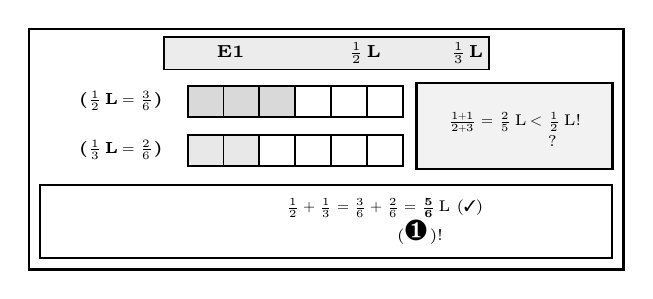
\begin{tikzpicture}[x=0.95cm, y=0.94cm, every node/.style={font=\scriptsize, text=black}]
  \draw[black, line width=0.95pt] (0,0) rectangle (7.95,3.25);
  \node[fill=gray!15, draw=black, line width=0.6pt, inner sep=2pt, font=\fontsize{6.3pt}{8.0pt}\selectfont\bfseries] at (3.975,2.92) {បេសកកម្ម \en{E1}៖ ចាក់ទឹកត្នោតផ្អែម $\frac{1}{2}\unit{L}$ បញ្ចូលជាមួយ $\frac{1}{3}\unit{L}$};

  % Bar 1/2 (3 of 6 cells, width 0.48 each -> 2.88 total from x=2.12 to 5.00)
  \node[anchor=west, font=\fontsize{5.8pt}{7.4pt}\selectfont\bfseries] at (0.14,2.28) {ដបទី១ ($\frac{1}{2}\unit{L}=\frac{3}{6}$)};
  \foreach \i in {0,1,2} { \fill[gray!30] (2.12+\i*0.48, 2.06) rectangle (2.12+\i*0.48+0.48, 2.48); }
  \foreach \i in {0,...,5} { \draw[black, line width=0.7pt] (2.12+\i*0.48, 2.06) rectangle (2.12+\i*0.48+0.48, 2.48); }

  % Bar 1/3 (2 of 6 cells)
  \node[anchor=west, font=\fontsize{5.8pt}{7.4pt}\selectfont\bfseries] at (0.14,1.62) {ដបទី២ ($\frac{1}{3}\unit{L}=\frac{2}{6}$)};
  \foreach \i in {0,1} { \fill[gray!18] (2.12+\i*0.48, 1.40) rectangle (2.12+\i*0.48+0.48, 1.82); }
  \foreach \i in {0,...,5} { \draw[black, line width=0.7pt] (2.12+\i*0.48, 1.40) rectangle (2.12+\i*0.48+0.48, 1.82); }

  % Paradox comparison box on right (generous width 2.60 units)
  \draw[black, line width=0.8pt, fill=gray!10] (5.18,1.36) rectangle (7.80,2.52);
  \node[align=center, font=\fontsize{5.6pt}{7.3pt}\selectfont] at (6.49,1.94) {\textbf{អន្ទាក់បូកភាគបែង៖}\\$\frac{1+1}{2+3} = \frac{2}{5}\unit{L} < \frac{1}{2}\unit{L}$!\\ចាក់ថែម តិចជាងមុន?};

  % Bottom conclusion bar (2 clean centered lines inside box)
  \draw[black, line width=0.75pt] (0.15,0.16) rectangle (7.80,1.14);
  \node[align=center, font=\fontsize{5.6pt}{7.3pt}\selectfont] at (3.975,0.65) {\textbf{ឯកតារួម ៦ ក្រឡាស្មើគ្នា៖} $\frac{1}{2} + \frac{1}{3} = \frac{3}{6} + \frac{2}{6} = \mathbf{\frac{5}{6}\unit{L}}$ (\ding{51})\\\textbf{ច្បាប់មាស៖ ហាម}បូកភាគបែងនឹងភាគបែងជាដាច់ខាត (\cnum{1})!};
\end{tikzpicture}}

% ២. E2 POE 1 & POE 2: ស្តង់ដារសញ្ញាភាគបែង និងមេដែកផ្គុំគូផ្ទុយ-ភាគបែងដូចគ្នា (ទំ.៦-៧)
\newcommand{\figGroupingRATADD}{%
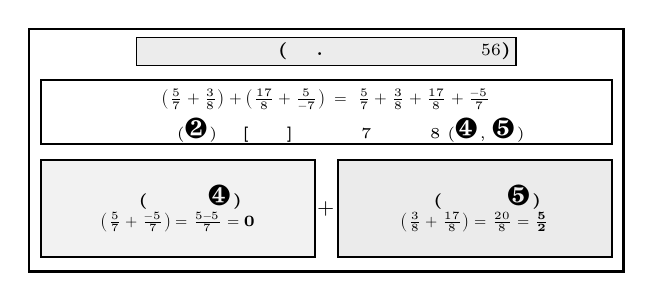
\begin{tikzpicture}[x=0.95cm, y=0.92cm, every node/.style={font=\scriptsize, text=black}]
  \draw[black, line width=0.95pt] (0,0) rectangle (7.95,3.35);
  \node[fill=gray!15, draw=black, line width=0.6pt, inner sep=2pt, font=\fontsize{6.2pt}{7.9pt}\selectfont\bfseries] at (3.975,3.04) {មេដែកលក្ខណៈត្រឡប់ និងផ្គុំ (គំរូទំ.៧ គ៖ គណនាដោយមិនបាច់រកភាគបែងរួម $56$)};

  % Step 1: Original expression with sign standardized
  \draw[black, line width=0.75pt] (0.16,1.76) rectangle (7.79,2.64);
  \node[font=\fontsize{5.9pt}{7.6pt}\selectfont] at (3.975,2.38) {$\left(\frac{5}{7} + \frac{3}{8}\right) + \left(\frac{17}{8} + \frac{5}{-7}\right) \;=\; \frac{5}{7} + \frac{3}{8} + \frac{17}{8} + \frac{-5}{7}$};
  \node[font=\fontsize{5.5pt}{7.1pt}\selectfont] at (3.975,1.96) {រុញដកឡើងលើ (\cnum{2}) រួច \textbf{[គូសភ្ជាប់]} ផ្គុំគូភាគបែង $7$ និងគូភាគបែង $8$ (\cnum{4}, \cnum{5})};

  % Two magnet boxes below
  \draw[black, line width=0.8pt, fill=gray!10] (0.16,0.20) rectangle (3.82,1.54);
  \node[align=center, font=\fontsize{5.7pt}{7.3pt}\selectfont] at (1.99,0.87) {\textbf{គូទី១ (គូផ្ទុយសូន្យ \cnum{4})៖}\\$\left(\frac{5}{7} + \frac{-5}{7}\right) = \frac{5-5}{7} = \mathbf{0}$};

  \node[font=\footnotesize\bfseries] at (3.975,0.87) {$+$};

  \draw[black, line width=0.8pt, fill=gray!16] (4.13,0.20) rectangle (7.79,1.54);
  \node[align=center, font=\fontsize{5.7pt}{7.3pt}\selectfont] at (5.96,0.87) {\textbf{គូទី២ (ភាគបែងដូចគ្នា \cnum{5})៖}\\$\left(\frac{3}{8} + \frac{17}{8}\right) = \frac{20}{8} = \mathbf{\frac{5}{2}}$};
\end{tikzpicture}}

% ៣. E4 Worked Example: អន្ទាក់ចំនួនចម្រុះអវិជ្ជមាន (-3 3/5) + (3 7/4) (ទំ.៦)
\newcommand{\figMixedTrapRATADD}{%
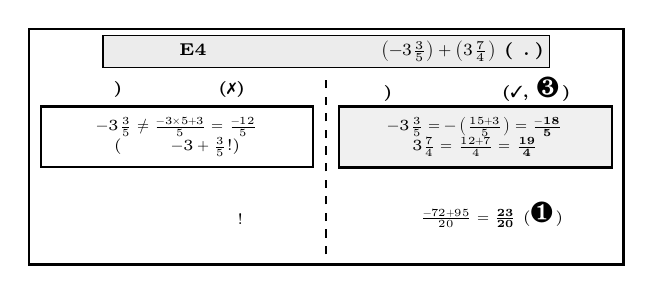
\begin{tikzpicture}[x=0.95cm, y=0.92cm, every node/.style={font=\scriptsize, text=black}]
  \draw[black, line width=0.95pt] (0,0) rectangle (7.95,3.25);
  \node[fill=gray!15, draw=black, line width=0.6pt, inner sep=2pt, font=\fontsize{6.2pt}{7.9pt}\selectfont\bfseries] at (3.975,2.94) {កាតស៊ើបអង្កេត \en{E4}៖ អន្ទាក់សញ្ញាចំនួនចម្រុះអវិជ្ជមាន $\left(-3\frac{3}{5}\right) + \left(3\frac{7}{4}\right)$ (ទំ.៦)};

  \draw[black, dashed, line width=0.65pt] (3.975,0.14) -- (3.975,2.62);

  % Left: Trap
  \node[font=\fontsize{5.8pt}{7.4pt}\selectfont\bfseries] at (1.98,2.42) {១) ច្រឡំផ្ដាច់សញ្ញាដក (\ding{55})};
  \draw[black, line width=0.75pt] (0.16,1.34) rectangle (3.80,2.18);
  \node[align=center, font=\fontsize{5.6pt}{7.2pt}\selectfont] at (1.98,1.76) {$-3\frac{3}{5} \neq \frac{-3\times 5 + 3}{5} = \frac{-12}{5}$\\(ច្រឡំគិតថា $-3 + \frac{3}{5}$!)};
  \node[align=center, font=\fontsize{5.5pt}{7.0pt}\selectfont] at (1.98,0.68) {សញ្ញាដកនៅមុខចំនួនចម្រុះ\\គ្របលើ\textbf{ទាំងផ្នែកគត់ ទាំងប្រភាគ}!};

  % Right: Correct
  \node[font=\fontsize{5.8pt}{7.4pt}\selectfont\bfseries] at (5.96,2.42) {២) វិធីបំប្លែងត្រឹមត្រូវ (\ding{51}, \cnum{3})};
  \draw[black, line width=0.85pt, fill=gray!12] (4.14,1.34) rectangle (7.79,2.18);
  \node[align=center, font=\fontsize{5.6pt}{7.2pt}\selectfont] at (5.965,1.76) {$-3\frac{3}{5} = -\left(\frac{15+3}{5}\right) = \mathbf{\frac{-18}{5}}$\\$3\frac{7}{4} = \frac{12+7}{4} = \mathbf{\frac{19}{4}}$};
  \node[align=center, font=\fontsize{5.6pt}{7.2pt}\selectfont] at (5.965,0.68) {ផលបូក៖ $\frac{-72 + 95}{20} = \mathbf{\frac{23}{20}}$ (\cnum{1})};
\end{tikzpicture}}

% ៤. E5 Diagnostic Cards A-D
\newcommand{\figExitCardsRATADD}{%
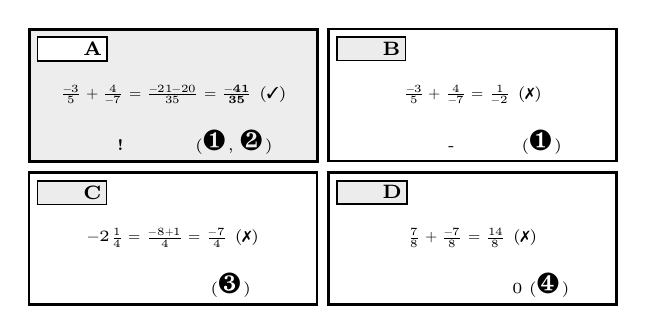
\begin{tikzpicture}[x=0.95cm, y=0.92cm, every node/.style={font=\scriptsize, text=black}]
  \draw[black, line width=1.1pt, fill=gray!14] (0,1.98) rectangle (3.85,3.80);
  \node[anchor=north west, fill=white, draw=black, line width=0.6pt, inner sep=1.8pt] at (0.10,3.70) {\textbf{ជម្រើស \en{A}}};
  \node[font=\fontsize{5.7pt}{7.4pt}\selectfont] at (1.925,2.90) {$\frac{-3}{5} + \frac{4}{-7} = \frac{-21-20}{35} = \mathbf{\frac{-41}{35}}$ (\ding{51})};
  \node[font=\fontsize{5.6pt}{7.2pt}\selectfont] at (1.925,2.24) {\textbf{ត្រឹមត្រូវ!} រុញដកឡើងលើសិន (\cnum{1}, \cnum{2})};

  \draw[black, line width=0.9pt] (4.00,1.98) rectangle (7.85,3.80);
  \node[anchor=north west, fill=gray!15, draw=black, line width=0.6pt, inner sep=1.8pt] at (4.10,3.70) {\textbf{ជម្រើស \en{B}}};
  \node[font=\fontsize{5.7pt}{7.4pt}\selectfont] at (5.925,2.90) {$\frac{-3}{5} + \frac{4}{-7} = \frac{1}{-2}$ (\ding{55})};
  \node[font=\fontsize{5.6pt}{7.2pt}\selectfont] at (5.925,2.24) {អន្ទាក់បូកភាគយក-ភាគបែងដាច់គ្នា (\cnum{1})};

  \draw[black, line width=0.9pt] (0,0) rectangle (3.85,1.82);
  \node[anchor=north west, fill=gray!15, draw=black, line width=0.6pt, inner sep=1.8pt] at (0.10,1.72) {\textbf{ជម្រើស \en{C}}};
  \node[font=\fontsize{5.7pt}{7.4pt}\selectfont] at (1.925,0.92) {$-2\frac{1}{4} = \frac{-8+1}{4} = \frac{-7}{4}$ (\ding{55})};
  \node[font=\fontsize{5.6pt}{7.2pt}\selectfont] at (1.925,0.26) {ច្រឡំសញ្ញាដកលើចំនួនចម្រុះ (\cnum{3})};

  \draw[black, line width=0.9pt] (4.00,0) rectangle (7.85,1.82);
  \node[anchor=north west, fill=gray!15, draw=black, line width=0.6pt, inner sep=1.8pt] at (4.10,1.72) {\textbf{ជម្រើស \en{D}}};
  \node[font=\fontsize{5.7pt}{7.4pt}\selectfont] at (5.925,0.92) {$\frac{7}{8} + \frac{-7}{8} = \frac{14}{8}$ (\ding{55})};
  \node[font=\fontsize{5.6pt}{7.2pt}\selectfont] at (5.925,0.26) {ភ្លេចថាគូចំនួនផ្ទុយបូកគ្នាស្មើ $0$ (\cnum{4})};
\end{tikzpicture}}

\begin{document}
\fontsize{10pt}{15.2pt}\selectfont

% -------------------- ក្បាលកិច្ចតែងការ --------------------
\begin{center}
  {\muol\fontsize{11pt}{16pt}\selectfont ព្រះរាជាណាចក្រកម្ពុជា}\\[2pt]
  {\muol\fontsize{10pt}{15pt}\selectfont ជាតិ សាសនា ព្រះមហាក្សត្រ}\\[1pt]
  \khmflourish
\end{center}

\vspace{-24pt}
{\muol\fontsize{9.5pt}{12.5pt}\selectfont
មន្ទីរអប់រំ យុវជន និងកីឡា ខេត្តកំពង់ធំ\\
ការិយាល័យអប់រំ យុវជន និងកីឡា ស្រុកកំពង់ស្វាយ\\
អនុវិទ្យាល័យព្រះក្រសាំង}

\vspace{1pt}
\begin{center}
  {\muol\fontsize{10pt}{14pt}\selectfont កិច្ចតែងការបង្រៀន}
\end{center}
\vspace{0pt}

% -------------------- ព័ត៌មានទូទៅ --------------------
{\renewcommand{\arraystretch}{0.98}
\hspace*{3.1cm}%
\begin{tabular}{@{}l l L{11.0cm}@{}}
  - \hspace{0.35cm} មុខវិជ្ជា & : & គណិតវិទ្យា ថ្នាក់ទី៨ (ពីជគណិត) \\
  - \hspace{0.35cm} ចំណងជើងមេរៀន & : & មេរៀនទី១៖ ចំនួនសនិទាន \\
  - \hspace{0.35cm} ចំណងជើងរង & : & ៣.១. ប្រមាណវិធីបូក និង ៣.២. លក្ខណៈនៃវិធីបូកចំនួនសនិទាន (ទំ.៥–៧) \\
  - \hspace{0.35cm} រយៈពេល & : & ១ ម៉ោងសិក្សា (៥០ នាទី) \\
  - \hspace{0.35cm} បង្រៀនដោយ & : & ហុក ប៊ុនថែន \\
  - \hspace{0.35cm} កាលបរិច្ឆេទ & : & ថ្ងៃពុធ ទី១៨ ខែវិច្ឆិកា ឆ្នាំ២០២៦ \\
\end{tabular}

\vspace{2pt}

% -------------------- I. វត្ថុបំណង --------------------
\textbf{I.} {\muol វត្ថុបំណង}\\[1pt]
\hspace*{0.55cm}%
\begin{tabular}{@{}l l L{14.2cm}@{}}
  \wcirc \hspace{0.25cm} វិជ្ជាសម្បទា & : & សិស្សប្រាប់រូបមន្តបូកចំនួនសនិទាន ($\frac{a}{b}+\frac{c}{b}=\frac{a+c}{b}$, $\frac{a}{b}+\frac{c}{d}=\frac{ad+bc}{bd}$) និងលក្ខណៈទាំង ៧ នៃវិធីបូកចំនួនសនិទាន (ត្រឡប់ ផ្គុំ ធាតុណឺត $0$ និងចំនួនផ្ទុយ) បានត្រឹមត្រូវតាមសៀវភៅគោល (ទំ.៥–៧) ។ \\
  \wcirc \hspace{0.25cm} បំណិនសម្បទា & : & សិស្សគណនាផលបូកចំនួនសនិទាន (ប្រភាគមានសញ្ញា ចំនួនចម្រុះ ចំនួនទសភាគ) និងចេះប្រើលក្ខណៈត្រឡប់-ផ្គុំដើម្បីគណនាផលបូករហ័សដោយដៃលើសន្លឹកកិច្ចការបានត្រឹមត្រូវ ។ \\
  \wcirc \hspace{0.25cm} ចរិយាសម្បទា & : & សិស្សមានទម្លាប់ពិនិត្យសញ្ញាភាគបែង និងប៉ាន់ស្មានទំហំលទ្ធផលដោយប្រុងប្រយ័ត្ន ជៀសវាងកំហុសបូកភាគបែងនឹងភាគបែង ក្នុងការដោះស្រាយបញ្ហាប្រចាំថ្ងៃ ។ \\
\end{tabular}

\vspace{2pt}

% -------------------- II. សម្ភារៈឧបទេស --------------------
\textbf{II.} {\muol សម្ភារៈឧបទេស}\\[1pt]
\hspace*{0.55cm}$\bullet$ \hspace{0.35cm} សៀវភៅសិក្សាគោលគណិតវិទ្យាថ្នាក់ទី៨ (ទំ.៥–៧) ក្ដារខៀន ដីស និងសន្លឹកកិច្ចការសិស្ស ស-ខ្មៅ (\en{Worksheet\_RAT\_ADD} ទំព័រ ១–២ គ្មានស្លាយ \en{LCD} គ្មានម៉ាស៊ីនគិតលេខ)

\vspace{2pt}

% -------------------- III. វិធីសាស្រ្តបង្រៀន --------------------
\textbf{III.} {\muol វិធីសាស្រ្តបង្រៀន}\\[1pt]
\hspace*{0.45cm}%
\begin{tabular}{@{}l l L{14.85cm}@{}}
  $\bullet$ \hspace{0.25cm} គោលវិធី & : & សិស្សមជ្ឈមណ្ឌល (បង្រៀនតាមសន្លឹកកិច្ចការស៊ើបអង្កេតជាដៃគូ និងក្ដារខៀន គ្មាន \en{LCD}) \\
  $\bullet$ \hspace{0.25cm} យុទ្ធវិធីបង្រៀន & : & គំរូ \en{5Es} រួមបញ្ចូលបន្ទះក្រឡាឯកតារួម \en{(POE)} និងយុទ្ធសាស្ត្រមេដែកផ្គុំគូផ្ទុយ-ភាគបែងដូចគ្នា \\
\end{tabular}
}

\vspace{2pt}

% -------------------- IV. ដំណើរការបង្រៀន --------------------
\textbf{IV.} {\muol ដំណើរការបង្រៀន}

\vspace{1pt}

\renewcommand{\arraystretch}{1.15}
\begin{longtable}{|L{5.50cm}|L{7.90cm}|L{4.80cm}|}
\hline
\rowcolor{headgray}
\multicolumn{1}{|c|}{\muol សកម្មភាពគ្រូ} &
\multicolumn{1}{c|}{\muol ខ្លឹមសារមេរៀន} &
\multicolumn{1}{c|}{\muol សកម្មភាពសិស្ស} \\
\hline
\endfirsthead

\hline
\rowcolor{headgray}
\multicolumn{1}{|c|}{\muol សកម្មភាពគ្រូ} &
\multicolumn{1}{c|}{\muol ខ្លឹមសារមេរៀន} &
\multicolumn{1}{c|}{\muol សកម្មភាពសិស្ស} \\
\hline
\endhead

\hline
\endfoot

\hline
\endlastfoot

% ==================== ជំហានទី១ (2min) ====================
\stepheader{ជំហានទី១ \enbf{(}រដ្ឋបាលថ្នាក់\enbf{)}}
$\bullet$ ពិនិត្យអវត្តមាន អនាម័យ និងសណ្ដាប់ធ្នាប់ថ្នាក់រៀន \timenote{(2 min)}\par\vspace{2pt}
$\bullet$ ចែក \textbf{សន្លឹកកិច្ចការសិស្ស (\en{Worksheet\_RAT\_ADD})} ម្នាក់ ១ សន្លឹក (ផ្កាប់ទុកសិន)
&
$\bullet$ រដ្ឋបាលថ្នាក់ និងការរៀបចំដៃគូសិក្សា (២ នាក់ក្នុង ១ តុ)\par\vspace{2pt}
$\bullet$ សន្លឹកកិច្ចការសិស្ស ស-ខ្មៅ ២ ទំព័រ សម្រាប់បំពេញតាមជំហានមេរៀន
&
$\circ$ ប្រធានថ្នាក់រាយការណ៍អវត្តមាន\par\vspace{2pt}
$\circ$ ទទួលសន្លឹកកិច្ចការ ដាក់ផ្កាប់លើតុ \\[3pt]
\hline

% ==================== ជំហានទី២ (9min: <=3 + 3 + E1 3) ====================
\stepheader{ជំហានទី២ \enbf{(}កិច្ចការផ្ទះ \enbf{+} ទំនាក់ទំនងមេរៀនថ្មី\enbf{)}}
\timenote{កំណែកិច្ចការផ្ទះ ($\le 3\unit{min}$)}\par\vspace{2pt}
$\bullet$ ហៅសិស្ស ២ នាក់ឡើងសរសេរចម្លើយកិច្ចការផ្ទះចំណុច ២.៣ លើក្ដារខៀន
&
\textbf{១. កំណែកិច្ចការផ្ទះ (ចំណុច ២.៣ លក្ខណៈចំនួនសនិទាន)៖}\par\vspace{2pt}
$\bullet$ \textbf{ក.} $\dfrac{-18}{45} = \dfrac{14}{-35} = \dfrac{-2}{5}$ \;;\; $\dfrac{-24}{-56} = \dfrac{15}{35} = \dfrac{3}{7}$\par\vspace{2pt}
$\bullet$ \textbf{ខ.} $\dfrac{5}{-8} = \dfrac{-5}{8} = \dfrac{-25}{40} < \dfrac{-3}{5} = \dfrac{-24}{40}$
&
$\circ$ តំណាងសិស្សឡើងកែលើក្ដារខៀន\par\vspace{2pt}
$\circ$ សិស្សផ្ទៀងផ្ទាត់ និងកែតម្រូវចូលសៀវភៅ \\[3pt]

\timenote{រំលឹកមេរៀនទាក់ទង (3 min)}\par\vspace{2pt}
$\bullet$ សួររំលឹកការបូកចំនួនគត់រ៉ឺឡាទីប និងការរកភាគបែងរួមតូចបំផុត \en{(PPCM)}៖\par\vspace{2pt}
\hspace*{0.3em}-- សំណួរ៖ «តើ $(-21) + (-20)$ និង $(-72) + 95$ ស្មើប៉ុន្មាន? តើ \en{PPCM}$(4,6,3)$ ស្មើប៉ុន្មាន?»
&
\textbf{២. រំលឹកមូលដ្ឋានគ្រឹះមុនមេរៀនថ្មី៖}\par\vspace{2pt}
$\bullet$ បូកចំនួនគត់រ៉ឺឡាទីប៖ $(-21)+(-20) = -41$ \;;\; $(-72)+95 = +23$\par\vspace{2pt}
$\bullet$ ភាគបែងរួមតូចបំផុត៖ $\text{\en{PPCM}}(4,6,3) = 12$ \;;\; សញ្ញា៖ $\frac{a}{-b} = \frac{-a}{b}$
&
$\circ$ ឆ្លើយផ្ទាល់មាត់៖ $-41$, $+23$ និង $\text{\en{PPCM}}(4,6,3)=12$ \\[3pt]

\fiveE{E1 - Engage} \timenote{(3 min)}\par\vspace{2pt}
$\bullet$ ឱ្យសិស្សផ្ងារសន្លឹកកិច្ចការទំព័រទី១ អានបេសកកម្ម \en{E1}៖ «ពូសុខចាក់ទឹកត្នោតផ្អែម $\frac{1}{2}\unit{L}$ បញ្ចូលជាមួយ $\frac{1}{3}\unit{L}$ ។ សិស្សម្នាក់សរសេរ $\frac{1}{2}+\frac{1}{3}=\frac{2}{5}\unit{L}$»\par\vspace{2pt}
\hspace*{0.3em}-- សំណួរបំផុស៖ «តើ $\frac{2}{5}\unit{L}$ ធំជាង ឬតូចជាងកន្លះលីត្រ ($\frac{1}{2}\unit{L}$)? ហេតុអ្វីចាក់ថែម បែរជាតិចជាងមុន?»
&
\textbf{៣. បេសកកម្ម \en{E1} — អន្ទាក់ទឹកត្នោតផ្អែម៖}\par\vspace{2pt}
$\bullet$ បើបូកភាគបែង៖ $\dfrac{1+1}{2+3} = \dfrac{2}{5} = 0.4\unit{L} < 0.5\unit{L}$ (មិនសមហេតុផល!)\par\vspace{2pt}
$\bullet$ ភ្ជាប់ចូលមេរៀនថ្មី៖ \textbf{៣.១. ប្រមាណវិធីបូក និង ៣.២. លក្ខណៈនៃវិធីបូក}
&
$\circ$ គូសធីកការទស្សន៍ទាយលើសន្លឹកកិច្ចការ និងភ្ញាក់ផ្អើលពេលឃើញ $\frac{2}{5} < \frac{1}{2}$! \\[3pt]

& \cfig{\figEngageRATADD} & \\[3pt]
\hline

% ==================== ជំហានទី៣ (17min: E2 11 + E3 6) ====================
\stepheader{ជំហានទី៣ \enbf{(}ខ្លឹមសារមេរៀនថ្មី\enbf{)}}
\fiveE{E2 - Explore} \timenote{(11 min)}\par\vspace{2pt}
$\bullet$ សរសេរចំណងជើងមេរៀនលើក្ដារខៀន និងណែនាំ \textbf{សកម្មភាពទី១ (\en{POE 1})} លើសន្លឹកកិច្ចការ (ទំ.៥–៦)
&
\textbf{៣. ប្រមាណវិធីបូកនិងដកនៃចំនួនសនិទាន}\par\vspace{2pt}
\textbf{៣.១. ប្រមាណវិធីបូក (ទំ.៥–៦) — \en{POE 1}៖}\par\vspace{2pt}
$\bullet$ ភាគបែងដូចគ្នា៖ $\dfrac{9}{5}+\dfrac{7}{5}=\dfrac{16}{5}$ \;;\; $\dfrac{3}{7}+\dfrac{-5}{7}=\dfrac{3-5}{7}=\dfrac{-2}{7}$
&
$\circ$ កត់ចំណងជើងមេរៀន និងពិភាក្សាជាដៃគូលើប្រភាគភាគបែងដូចគ្នា \\[3pt]

$\bullet$ ឱ្យដៃគូពិនិត្យករណីសញ្ញាដកនៅភាគបែង និងករណីភាគបែងខុសគ្នា (ទំ.៥ ខ, ឃ)
&
$\bullet$ រុញដកពីភាគបែងឡើងលើសិន៖ $\dfrac{-3}{8}+\dfrac{5}{-8} = \dfrac{-3}{8}+\dfrac{-5}{8} = \dfrac{-8}{8} = -1$\par\vspace{2pt}
$\bullet$ ភាគបែងខុសគ្នា៖ $3.5+\dfrac{79}{10}=\dfrac{35+79}{10}=\dfrac{57}{5}$ \;;\; $\dfrac{-3}{5}+\dfrac{4}{-7}=\dfrac{-21-20}{35}=\dfrac{-41}{35}$
&
$\circ$ គណនាលំហាត់គំរូទី១ (ក–ឃ ទំ.៥–៦) លើសន្លឹកកិច្ចការ \\[3pt]

$\bullet$ ណែនាំ \textbf{សកម្មភាពទី២ (\en{POE 2} — មេដែកផ្គុំគូផ្ទុយ និងភាគបែងដូចគ្នា ទំ.៦–៧)}៖\par\vspace{2pt}
\hspace*{0.3em}-- \textbf{ទស្សន៍ទាយ (\en{P})៖} «តើចាំបាច់រកភាគបែងរួម $56$ ចំពោះ $\left(\frac{5}{7}+\frac{3}{8}\right)+\left(\frac{17}{8}+\frac{5}{-7}\right)$ ឬអាចផ្គុំគូរហ័ស?»
&
\textbf{៣.២. លក្ខណៈនៃវិធីបូក (ទំ.៦–៧) — \en{POE 2}៖}\par\vspace{2pt}
$\bullet$ ប្ដូរ $\dfrac{5}{-7} = \dfrac{-5}{7}$ រួចប្រើលក្ខណៈត្រឡប់ និងលក្ខណៈផ្គុំ៖\par\vspace{2pt}
$\left(\dfrac{5}{7}+\dfrac{-5}{7}\right) + \left(\dfrac{3}{8}+\dfrac{17}{8}\right) = 0 + \dfrac{20}{8} = \graybox{$\dfrac{5}{2}$}$
&
$\circ$ រកឃើញថាការផ្គុំគូចំនួនផ្ទុយ $\frac{5}{7}+\frac{-5}{7}=0$ និងគូភាគបែង $8$ លឿនជាងការតម្រូវភាគបែង $56$ ឆ្ងាយណាស់! \\[3pt]

& \cfig{\figGroupingRATADD} & \\[3pt]

\fiveE{E3 - Explain} \timenote{(6 min)}\par\vspace{2pt}
$\bullet$ ហៅតំណាងដៃគូឡើងបង្គុំរូបមន្តទូទៅនៃប្រមាណវិធីបូក (ទំ.៥) លើក្ដារខៀន
&
\textbf{សំយោគបញ្ញត្តិ និងធនាគារហេតុផល \en{B\&W} (\cnum{1}--\cnum{5})៖}\par\vspace{2pt}
$\bullet$ \textbf{ជាទូទៅ (ទំ.៥)៖} $\dfrac{a}{b}+\dfrac{c}{d} = \dfrac{ad+bc}{bd}$ \;;\; \textbf{សម្គាល់៖} $\dfrac{a}{b}+\dfrac{c}{b} = \dfrac{a+c}{b}$
&
$\circ$ តំណាងដៃគូឡើងបកស្រាយរូបមន្តបូកប្រភាគលើក្ដារខៀន \\[3pt]

$\bullet$ សង្ខេបលក្ខណៈទី១ ដល់ទី៤ នៃវិធីបូកចំនួនសនិទាន (ទំ.៦)
&
$\bullet$ \textbf{លក្ខណៈទី១–៤ (ទំ.៦)៖} (១) ផលបូកជាចំនួនសនិទាន; (២) \textbf{ត្រឡប់} $\frac{a}{b}+\frac{c}{d}=\frac{c}{d}+\frac{a}{b}$; (៣) \textbf{ផ្គុំ} $(\frac{a}{b}+\frac{c}{d})+\frac{e}{f}=\frac{a}{b}+(\frac{c}{d}+\frac{e}{f})$; (៤) \textbf{ធាតុណឺត} $\frac{a}{b}+0=\frac{a}{b}$
&
$\circ$ បំពេញប្រអប់រូបមន្តផ្នែកទី២ លើសន្លឹកកិច្ចការ \\[3pt]

$\bullet$ បន្តសង្ខេបលក្ខណៈទី៥ ដល់ទី៧ (ចំនួនផ្ទុយ និងសញ្ញាដកពីរជាន់ ទំ.៦)
&
$\bullet$ \textbf{លក្ខណៈទី៥–៧ (ទំ.៦)៖} (៥) \textbf{ចំនួនផ្ទុយ} $\frac{a}{b}+\left(-\frac{a}{b}\right)=0$; (៦) សម្រួលតួដូចគ្នា; (៧) $-\left(-\frac{a}{b}\right)=\frac{a}{b}$
&
$\circ$ កត់ត្រាលក្ខណៈចំនួនផ្ទុយ និងសញ្ញាដកពីរជាន់ \\[3pt]

$\bullet$ កត់ធនាគារហេតុផល \cnum{1}--\cnum{5} លើក្ដារខៀន សម្រាប់យោងពេលដោះស្រាយលំហាត់
&
\cnum{1} តម្រូវភាគបែងរួមជាមុន ទើបបូកភាគយក (រក្សាភាគបែងទុកដដែល) ។\par\vspace{1.5pt}
\cnum{2} បើភាគបែងអវិជ្ជមាន ត្រូវរុញសញ្ញាដកឡើងភាគយកសិន ($\frac{a}{-b}=\frac{-a}{b}$) ។\par\vspace{1.5pt}
\cnum{3} ចំនួនចម្រុះអវិជ្ជមាន៖ $-k\frac{r}{b} = -\frac{kb+r}{b}$ (ដកគ្របលើទាំងមូល) ។
&
$\circ$ ផ្ទៀងផ្ទាត់ធនាគារហេតុផល \cnum{1}--\cnum{3} លើសន្លឹកកិច្ចការ \\[3pt]

$\bullet$ បញ្ជាក់ហេតុផល \cnum{4}--\cnum{5} សម្រាប់ការគណនាផលបូករហ័សដោយមិនបាច់តម្រូវភាគបែងធំ
&
\cnum{4} គូចំនួនផ្ទុយបូកបញ្ចូលគ្នាស្មើសូន្យ៖ $\frac{a}{b}+\left(-\frac{a}{b}\right)=0$ ។\par\vspace{1.5pt}
\cnum{5} លក្ខណៈត្រឡប់-ផ្គុំ៖ ប្ដូរទីតាំងផ្គុំប្រភាគមានភាគបែងដូចគ្នា ឬគូផ្ទុយសិន ។
&
$\circ$ ធ្វើលំហាត់ត្រួតពិនិត្យរហ័សនៅបាតទំព័រទី១ \\[3pt]
\hline

% ==================== ជំហានទី៤ (20min: E4 10 + E5 10) ====================
\stepheader{ជំហានទី៤ \enbf{(}ពង្រឹង និងពង្រីកចំណេះដឹង\enbf{)}}
\fiveE{E4 - Elaborate} \timenote{(10 min)}\par\vspace{2pt}
$\bullet$ ឱ្យសិស្សបើកសន្លឹកកិច្ចការទំព័រទី២ (ផ្នែកទី៣) ស៊ើបអង្កេត \textbf{លំហាត់គំរូទី២} (ទំ.៦)៖\par\vspace{2pt}
\hspace*{0.3em}-- សង្កត់ធ្ងន់លើអន្ទាក់ $-3\frac{3}{5} = -\frac{18}{5}$ (មិនមែន $\frac{-12}{5}$ ទេ!)
&
\textbf{១. លំហាត់គំរូទី២ (ទំ.៦) និងលំហាត់គំរូផ្គុំ (ទំ.៧)៖}\par\vspace{2pt}
$\bullet$ \textbf{ក)} $\left(-3\dfrac{3}{5}\right)+\left(3\dfrac{7}{4}\right) = \dfrac{-18}{5}+\dfrac{19}{4} = \dfrac{-72+95}{20} = \graybox{$\dfrac{23}{20}$} \quad (\text{\cnum{3},\cnum{1}})$\par\vspace{2pt}
$\bullet$ \textbf{ខ)} $\left(\dfrac{-1}{4}\right)+\dfrac{5}{6}+\dfrac{7}{3} = \dfrac{-3+10+28}{12} = \graybox{$\dfrac{35}{12}$}$
&
$\circ$ បំពេញជំហានគណនា ក និង ខ ក្នុងតារាង \en{E4} និងសរសេរលេខហេតុផល \\[3pt]

$\bullet$ ណែនាំការតម្រឹមចំណុចទសភាគ និងការអនុវត្តលក្ខណៈផ្គុំ (ទំ.៦ គ និងទំ.៧ ក)
&
$\bullet$ \textbf{គ)} $437.56+127.95=\mathbf{565.51}$ (តម្រឹមចំណុចទសភាគឱ្យត្រង់ជួរឈរ)\par\vspace{2pt}
$\bullet$ \textbf{ឃ) ប្រើលក្ខណៈផ្គុំ (ទំ.៧ ក)៖} $\left(\dfrac{5}{6}+\dfrac{7}{3}\right)+\dfrac{5}{3} = \dfrac{5}{6}+\left(\dfrac{7}{3}+\dfrac{5}{3}\right) = \dfrac{5}{6}+4 = \graybox{$\dfrac{29}{6}$}$
&
$\circ$ ឆ្លើយសំណួរ \en{EIA Looking-Back} ពីមូលហេតុដែល $-3\frac{3}{5}=-\frac{18}{5}$ \\[3pt]

& \cfig{\figMixedTrapRATADD} & \\[3pt]

\fiveE{E5 - Evaluate} \timenote{(10 min)}\par\vspace{2pt}
$\bullet$ ឱ្យសិស្សធ្វើលំហាត់ \textbf{ប្រតិបត្តិ} (ទំ.៦ ក, ខ, គ) លើសន្លឹកកិច្ចការ រួចប្ដូរសន្លឹកផ្ទៀងផ្ទាត់ (\en{Pause-Review})
&
\textbf{២. ប្រតិបត្តិ (ទំ.៦ និងទំ.៧) និងចម្លើយបិទបេសកកម្ម \en{E1}៖}\par\vspace{2pt}
$\bullet$ ទំ.៦៖ ក) $\left(-\dfrac{21}{4}\right)+\left(-\dfrac{11}{4}\right)=\dfrac{-32}{4}=\mathbf{-8}$ \;;\; ខ) $2\dfrac{1}{4}+5\dfrac{1}{4}=\dfrac{30}{4}=\mathbf{\dfrac{15}{2}}$\par\vspace{2pt}
$\bullet$ គ) $2\dfrac{5}{8}+\left(-1\dfrac{1}{8}\right)+3\dfrac{7}{8} = \dfrac{21-9+31}{8} = \mathbf{\dfrac{43}{8}}$
&
$\circ$ គណនាប្រតិបត្តិទំ.៦ ដោយដៃ និងផ្ទៀងផ្ទាត់សញ្ញាជាដៃគូ \\[3pt]

$\bullet$ បន្តផ្ទៀងផ្ទាត់ \textbf{ប្រតិបត្តិ ទំ.៧} (ប្រើលក្ខណៈត្រឡប់ និងលក្ខណៈផ្គុំ)
&
$\bullet$ ទំ.៧៖ ក) $\left(\dfrac{7}{4}+\dfrac{8}{3}\right)+\dfrac{10}{3} = \dfrac{7}{4}+6 = \mathbf{\dfrac{31}{4}}$ \;;\; ខ) $\left(\dfrac{5}{4}+\dfrac{3}{8}\right)+\dfrac{15}{4} = 5+\dfrac{3}{8} = \mathbf{\dfrac{43}{8}}$
&
$\circ$ ផ្ទៀងផ្ទាត់ការផ្គុំគូភាគបែង $3$ និងគូភាគបែង $4$ ជាដៃគូ \\[3pt]

$\bullet$ ហៅតំណាងដៃគូឆ្លើយបិទបញ្ចប់បេសកកម្មទឹកត្នោតផ្អែម \en{E1}
&
$\bullet$ \textbf{បិទ \en{E1}៖} ទឹកត្នោតផ្អែមសរុបគឺ $\dfrac{1}{2}+\dfrac{1}{3}=\dfrac{3+2}{6}=\mathbf{\dfrac{5}{6}\unit{L}} > \dfrac{1}{2}\unit{L}$ (\cnum{1})!
&
$\circ$ តំណាងដៃគូបកស្រាយបិទបញ្ចប់បេសកកម្ម \en{E1} \\[3pt]

$\bullet$ វាយតម្លៃរហ័ស \textbf{៦០ វិនាទី}៖ ឱ្យសិស្សគូសវង់ជម្រើសត្រឹមត្រូវក្នុងប្រអប់ \en{A--D} និងបំពេញសំបុត្រចេញ
&
\textbf{៣. វិនិច្ឆ័យកំហុសរហ័ស (\en{A--D})៖} ចម្លើយត្រឹមត្រូវគឺ \graybox{\textbf{ជម្រើស \en{A}}} ($\frac{-41}{35}$) ។\par\vspace{2pt}
(\en{B} បូកភាគបែងខុសក្បួន; \en{C} ច្រឡំចំនួនចម្រុះអវិជ្ជមាន; \en{D} ភ្លេចចំនួនផ្ទុយស្មើ $0$)
&
$\circ$ គូសវង់ជម្រើស \en{A} និងកែតម្រូវកំហុសភ្លាមៗមុនបញ្ចប់ម៉ោង \\[3pt]

& \cfig{\figExitCardsRATADD} & \\[3pt]
\hline

% ==================== ជំហានទី៥ (<=2min) ====================
\stepheader{ជំហានទី៥ \enbf{(}កិច្ចការផ្ទះ \enbf{+} បណ្ដាំផ្ញើ\enbf{)}}
\timenote{ចំណាយពេលឱ្យតិចបំផុតកុំឱ្យលើស 2 min}\par\vspace{2pt}
$\bullet$ ណែនាំកិច្ចការផ្ទះនៅផ្នែកទី៥ នៃសន្លឹកកិច្ចការ (សៀវភៅពុម្ព ទំ.៧ និងទំ.១២ \#9) និងផ្ដាំផ្ញើឱ្យអានមុនចំណុច \textbf{៣.៣. ប្រមាណវិធីដកនៃចំនួនសនិទាន} (ទំ.៧–៨)
&
\centerline{\muol កិច្ចការផ្ទះ}\par\vspace{2pt}
$\bullet$ \textbf{លំហាត់ ១៖} គណនា រួចសម្រួល៖ ក) $\left(-\dfrac{1}{8}\right)+\left(2\dfrac{5}{9}\right)$ \quad ខ) $\dfrac{12}{25}+\left(-2\dfrac{5}{7}\right)$ \quad គ) $\left(-1\dfrac{3}{4}\right)+\dfrac{5}{-6}+\dfrac{7}{12}$\par\vspace{2pt}
$\bullet$ \textbf{លំហាត់ ២៖} គណនាដោយប្រើលក្ខណៈផ្គុំ៖ $\left(\dfrac{-3}{11}+\dfrac{5}{12}\right)+\left(\dfrac{7}{12}+\dfrac{3}{11}\right)$\par\vspace{2pt}
$\bullet$ \textbf{បណ្ដាំផ្ញើ៖} អានមុនចំណុច \textbf{៣.៣. ប្រមាណវិធីដកនៃចំនួនសនិទាន} (សៀវភៅពុម្ព ទំ.៧–៨) ។
&
$\circ$ កត់ត្រាកិច្ចការផ្ទះ និងទទួលបណ្ដាំផ្ញើដោយសណ្ដាប់ធ្នាប់ \\[3pt]
\end{longtable}

% -------------------- កាលបរិច្ឆេទ និងហត្ថលេខា --------------------
\vspace{2pt}
\hfill
\begin{minipage}{9.8cm}
  {\centering
    ថ្ងៃពុធ ៩កើត ខែកត្តិក ឆ្នាំមមី អដ្ឋស័ក ពុទ្ធសករាជ ២៥៧០\\[2pt]
    ត្រូវនឹងថ្ងៃទី១៨ ខែវិច្ឆិកា ឆ្នាំ២០២៦\\[3pt]
    {\muol គ្រូបង្រៀន}\par}
  \vspace{28pt}
  \hfill{\muol ហុក ប៊ុនថែន}\hspace*{1.4cm}
\end{minipage}

\end{document}
